\documentclass[11pt]{article}
\usepackage[margin=1in]{geometry}
\usepackage[T1]{fontenc}
\usepackage[utf8]{inputenc}
\usepackage{enumitem}
\usepackage{hyperref}
\usepackage{xurl}
\usepackage{amsmath}
\usepackage{upquote}
\usepackage{graphicx}
\usepackage{tikz}
\usetikzlibrary{arrows.meta, positioning, shapes.geometric}
\hypersetup{colorlinks=true, linkcolor=blue, urlcolor=blue}
\setlist{nosep,leftmargin=*}
\setlength{\parskip}{0.6em}
\setlength{\parindent}{0pt}

\title{SpaceAGORA\_RL Structure and Implementation Plan}
\date{June 4, 2026}

\begin{document}
\maketitle


\textbf{Reference code:} SpaceAGORA\_RL.jl/Reference Code/\\
\textbf{Target subsystem:} SpaceAGORA\_RL.jl\\


\section{Summary}

The reference ABTS code provides the source definitions for the paper's MDP, DDQN training loop, parallel worker protocol, baseline policy behavior, and evaluation metrics. The executable Python environment is coupled to the ABTS paths, CSV file exchange, mpi4py, PyTorch checkpoints, Python-specific Gym-like spaces, and local directory conventions.

The Julia implementation for use with SpaceAGORA will use the following reference-code elements:

\begin{enumerate}
\item The MDP contract:
\begin{itemize}
\item 9-feature paper observation schema.
\item Observation normalization bounds.
\item 13 discrete apoapsis delta-V actions.
\item Action sign convention and phi mapping.
\item Terminal, impact, out-of-drag-passage, and target-success semantics.
\item Reward terms and thermal corridor thresholds.

\end{itemize}
\item The DDQN mechanics:
\begin{itemize}
\item Online Q network and target Q network.
\item Epsilon-greedy action selection.
\item Double-DQN target calculation.
\item Adam optimizer settings.
\item Training cadence and target-update cadence.
\item Checkpoint/resume concept.

\end{itemize}
\item The parallel training protocol:
\begin{itemize}
\item Rank-0/master learner.
\item Worker rollout processes.
\item Workers sending transitions and episode summaries.
\item Master selecting the next action and training from replay.

\end{itemize}
\item The baseline/evaluation logic:
\begin{itemize}
\item AADS/NPC-style heat-corridor heuristic.
\item No-maneuver and random-action baselines.
\item Episode metrics: success, distance to target, thermal violations, total delta-V, number of maneuvers, number of passes, mission duration, heat-rate traces, action traces.
\end{itemize}
\end{enumerate}

The Julia implementation replaces the following reference-code runtime elements with SpaceAGORA-supported equivalents:

\begin{enumerate}
\item ABTS environment setup and subprocess/CSV simulation calls.
\item Local hard-coded directory paths.
\item Python \texttt{spaces} package.
\item PyTorch model/checkpoint code.
\item mpi4py bootstrap and network-address discovery.
\item Python-only logging and replay-memory CSV reconstruction.
\item Ad hoc deletion of checkpoint files during training.
\end{enumerate}

The implementation follows the structure already present in SpaceAGORA:

\begin{itemize}
\item \texttt{src/mission/operations/aerobraking\_policy/*} owns mission-level policy selection and already contains \texttt{DRLPolicyAdapterStub}.
\item \texttt{src/gnc/guidance/aerobraking/*} owns aerobraking strategy and guidance planning.
\item \texttt{src/gnc/control/aerobraking/*} owns tracking/execution.
\item \texttt{SpaceAGORA\_RL.jl} owns MDP construction, learning, evaluation, randomization, and artifacts.


\end{itemize}
\section{Reference-Code Adaptation Inventory}

\subsection{\texttt{make\_env.py}}

\paragraph{Adapt.}

Use existing SpaceAGORA values where possible, values below are reference.

\begin{itemize}
\item Phase targets and normalization scales:
\begin{itemize}
\item Walkout target apoapsis radius: 3900 km, normalization radius: 5000 km.
\item Endgame target apoapsis radius: 4906 km, normalization radius: 10100 km.
\item Main target apoapsis radius: 3900 km, normalization radius: 10100 km.
\item Campaign target apoapsis radius: 3900 km, normalization radius: 30000 km.

\end{itemize}
\item Mars constants used for paper-mode fixtures:
\begin{itemize}
\item Mars radius: 3.3962e6 m.
\item J2: 1.96045e-3.
\item Mu: 4.2828e13 m\textasciicircum{}3/s\textasciicircum{}2.
\item Exponential-atmosphere reference values: rho\_ref, h\_ref, H.
\item Gas constants and fixed-temperature values used in the reference implementation.

\end{itemize}
\item Paper observation schema and normalization:
\begin{itemize}
\item Drag-passage time normalized from 400 s to 1200 s.
\item Apoapsis radius normalized from Mars radius to phase-dependent \texttt{r\_norm}.
\item Periapsis altitude normalized from 85 km to 145 km.
\item Argument of periapsis normalized from 0 to pi.
\item RAAN normalized from 1.57 to 3.14 rad.
\item Inclination normalized from 1.39 to 1.75 rad.
\item Date ordinal normalized from 730486 to 731216.
\item Max density normalized from 0 to 1.5e-7 kg/m\textasciicircum{}3 in NN mode.
\item Max heat rate normalized from 0 to 0.5 W/cm\textasciicircum{}2 in NN mode.

\end{itemize}
\item Executable action table:
\begin{itemize}
\item \texttt{[-1.0, -0.5, -0.3, -0.2, -0.1, -0.05, 0.0, 0.05, 0.1, 0.2, 0.3, 0.5, 1.0]} m/s.
\item Negative actions lower periapsis through phi = 0.
\item Positive actions raise periapsis through phi = 180.
\item Zero action is index 7 in Julia 1-based indexing, corresponding to Python index 6.

\end{itemize}
\item Termination/reward rules:
\begin{itemize}
\item Success if \texttt{abs(ra - finalstate) <= 10 km}.
\item Impact if periapsis altitude is below the paper-mode lower threshold.
\item Out-of-drag-passage if periapsis altitude is above the paper-mode upper threshold.
\item Terminal if target reached, target undershot, impact/out-of-passage, or thermal violation in training mode.
\item Thermal corridor is 0.05 to 0.25 W/cm\textasciicircum{}2 while far from the target.
\item Above 0.25 W/cm\textasciicircum{}2 is disallowed near the target.
\item Thermal penalties: -4 for low/out-of-corridor, -5 for 0.30 to 0.45 W/cm\textasciicircum{}2, -6 for greater than 0.45 W/cm\textasciicircum{}2.
\item Success reward: \texttt{-floor(abs(ra - finalstate)/1000) * 2/5 + 10}.
\item Running reward:
\texttt{(1 - d\_cap\textasciicircum{}0.4) * (0.025 / (0.1 * sqrt(2*pi))) * exp(-0.5 * ((hr\_cap - 0.5)/0.1)\textasciicircum{}2) + (-0.1 - 0.1*deltav\_cap)}.
\end{itemize}
\end{itemize}

\paragraph{Rewrite.}

\begin{itemize}
\item \texttt{\_env\_setup}, \texttt{call\_ABTS}, CSV polling, file removal, and local path logic.
\item \texttt{\_getstate\_dragpassage} closed-form approximation, except for formula reference where paper parity is required.
\item Direct mutable environment fields become typed Julia structs.
\item Python \texttt{reset} and \texttt{step} signatures are replaced by the Julia backend contract.
\end{itemize}

\paragraph{Note.}

\begin{itemize}
\item The comment at the top of \texttt{make\_env.py} lists an older 11-action \texttt{[-1.5, ..., 1.5]} set. The actual executable DQN table is the 13-action \texttt{[-1, ..., 1]} set. The Julia implementation should use the executable 13-action table. [-1, -0.5, -0.3, -0.2, -0.1,-0.05, 0.0, 0.05, 0.1, 0.2, 0.3, 0.5, 1,] 
\end{itemize}


\subsection{\texttt{make\_env\_heuristic.py} and \texttt{DeterministicHeuristic.py}}

\paragraph{Adapt.}

\begin{itemize}
\item The heat-corridor heuristic becomes \texttt{tasks/aerobraking/baselines/aads\_heuristic.jl}.
\item The core rule is:
\begin{itemize}
\item Predict next heat rate with no maneuver.
\item If heat rate is inside 0.05 to 0.25 W/cm\textasciicircum{}2, use zero maneuver.
\item If heat rate is below the corridor, solve for a lowering maneuver that moves predicted heat rate toward 0.15 W/cm\textasciicircum{}2.
\item If heat rate is above the corridor, solve for a raising maneuver that moves predicted heat rate toward 0.15 W/cm\textasciicircum{}2.
\end{itemize}
\item The reference uses bisection over action magnitude, with fallback brackets of roughly 1, 3, and 6 m/s.
\end{itemize}

\paragraph{Rewrite.}

\begin{itemize}
\item Prediction calls the SpaceAGORA backend.
\item State reinitialization is represented as explicit backend state reset or reconstruction.
\end{itemize}


\subsection{\texttt{Algo.py}}

\paragraph{Adapt.}

\begin{itemize}
\item DDQN object responsibilities:
\begin{itemize}
\item online network;
\item target network;
\item replay memory;
\item epsilon schedule;
\item action selection;
\item observe/push transition;
\item train step;
\item target-network copy;
\item checkpoint save/load.

\end{itemize}
\item Training defaults:
\begin{itemize}
\item learning rate: 1e-4;
\item discount: 0.95;
\item batch size: 256;
\item train every 5 environment steps;
\item train after 10000 steps;
\item target update every 10000 train steps in the reference. The PDF specifies every 10000 global/environment steps. The selected cadence is stored in configuration and recorded in the run manifest.
\item gradient clipping norm: 10.
\item Adam epsilon: 1e-6 in the reference code. The PDF only says Adam; preserve this in paper-compatible mode unless experiments show it is not material.

\end{itemize}
\item Double-DQN target:
\begin{itemize}
\item action selection from the online network;
\item target value from the target network;
\item \texttt{target = reward + gamma * target\_q(next\_state, argmax\_online(next\_state))} for non-terminal transitions.
\end{itemize}
\end{itemize}

\paragraph{Rewrite.}

\begin{itemize}
\item PyTorch-specific code is rewritten in Flux/Optimisers or another selected Julia package or custom code.
\item The ActorCritic branch can be dropped from the first implementation because the paper uses PR-DDQN.
\item The \texttt{act} logic currently explores only before \texttt{train\_start} because of \texttt{self.num\_act\_steps < self.train\_start}. This appears inconsistent with a normal decaying epsilon policy. Implement the configured epsilon schedule deliberately, with tests.
\end{itemize}


\subsection{\texttt{Model.py}}

\paragraph{Adapt.}

\begin{itemize}
\item The reference model is a two-hidden-layer fully connected Q network.
\item Actual reference default is \texttt{n\_hidden=512}, but each hidden layer uses \texttt{2*n\_hidden}, giving 1024 units per hidden layer. This matches the PDF's two 1024-unit hidden layers.
\item Orthogonal initialization with zero biases is used in the reference.
\item ReLU activations are used.
\end{itemize}

\paragraph{Rewrite.}

\begin{itemize}
\item Port only the FC Q-network to Julia to match the paper:
\texttt{Dense(obs\_dim => 1024, relu)}, \texttt{Dense(1024 => 1024, relu)}, \texttt{Dense(1024 => n\_actions)}.
\item CNN and LSTM code are out of scope.
\end{itemize}


\subsection{\texttt{Replay.py}}

\paragraph{Adapt.}

\begin{itemize}
\item Replay buffer API:
\begin{itemize}
\item fixed capacity;
\item push transition;
\item random minibatch sampling;
\item terminal transitions omit next-state contribution.
\end{itemize}
\end{itemize}

\paragraph{Rewrite.}

\begin{itemize}
\item Do not keep the Python \texttt{deque} implementation.
\item Implement a typed circular buffer in Julia using contiguous arrays:
\begin{itemize}
\item \texttt{observations::Matrix\{Float32\}};
\item \texttt{actions::Vector\{Int\}};
\item \texttt{rewards::Vector\{Float32\}};
\item \texttt{next\_observations::Matrix\{Float32\}};
\item \texttt{terminated::Vector\{Bool\}};
\item \texttt{truncated::Vector\{Bool\}};
\item optional \texttt{info\_index::Vector\{Int\}} for metadata indexing.
\end{itemize}
\end{itemize}

\paragraph{Note.}

\begin{itemize}
\item The reference buffer does not distinguish \texttt{terminated} and \texttt{truncated}. The Julia implementation should use the split and map terminal flags into the DQN bootstrapping mask according to configuration.
\end{itemize}


\subsection{\texttt{Main\_DRL.py}}

\paragraph{Adapt.}

\begin{itemize}
\item Config keys and training-loop shape:
\begin{itemize}
\item max steps;
\item test episode count;
\item learning rate;
\item train frequency;
\item train start;
\item batch size;
\item discount;
\item replay size;
\item target update;
\item checkpoint frequency;
\item phase;
\item nominal/randomized mode;
\item output mode.

\end{itemize}
\item Parallel protocol:
\begin{itemize}
\item worker sends \texttt{(observation, result, action, next\_observation, first\_action, optional\_episode\_stats)};
\item master sends back \texttt{(new\_action, endloop)};
\item episode stats include episode length, reward, reached-goal flag, maneuver count, impact/out-of-passage flags, thermal violation count, distance to target, mission time, delta-V, heat-rate trace, action trace, apoapsis trace, periapsis trace, omega trace.
\end{itemize}
\end{itemize}

\paragraph{Rewrite.}

\begin{itemize}
\item Replace mpi4py with Julia \texttt{Distributed} as the default paper-replication worker backend.
\item Shell network-interface discovery, local checkpoint cleanup, and signal handlers are replaced by Julia script/runtime behavior.
\item Checkpoints are organized by run id and manifest rather than by deletion inside the training loop.
\end{itemize}


\subsection{\texttt{physics.py}}

Do not adapt, use SpaceAGORA native physics model


\subsection{\texttt{evaluation\_function.py}, \texttt{Evaluation.py}, \texttt{Draw.py}, logs, checkpoint}

\paragraph{Adapt.}

\begin{itemize}
\item Evaluation metrics and log fields:
\begin{itemize}
\item success/reached-goal count;
\item thermal violations;
\item impact/out-of-drag-passage;
\item target distance;
\item mission duration;
\item total delta-V;
\item maneuver count;
\item heat-rate/action/apoapsis/periapsis traces.
\end{itemize}
\end{itemize}

\paragraph{Rewrite.}

\begin{itemize}
\item Reports are produced as \texttt{DataFrames}, \texttt{CSV}, \texttt{Arrow}, and markdown/plots from Julia.
\end{itemize}


\subsection{\texttt{spaces/}, \texttt{misc/}, sbatch scripts}

\paragraph{Excluded files.}

\begin{itemize}
\item \texttt{spaces/} is a local Python Gym-like compatibility layer. Julia uses typed config and environment structs.
\item \texttt{misc/seeding.py} is replaced by Julia RNG ownership with explicit seeds.
\item \texttt{misc/utils.py} contains PyTorch helpers and is not needed for the first implementation.
\end{itemize}

\paragraph{Adapt.}

\begin{itemize}
\item sbatch scripts can inform future HPC examples, but write new scripts for Julia project commands and current SpaceAGORA paths.


\end{itemize}
\section{Updated Target Folder Structure}

Planned structure inside \texttt{SpaceAGORA\_RL.jl}:

\begin{verbatim}
SpaceAGORA_RL.jl/
  Project.toml
  Manifest.toml
  README.md
  src/
    SpaceAGORA_RL.jl

    core/
      mdp_interface.jl
      backend_interface.jl
      policy_interface.jl
      transition_schema.jl

    runtime/
      config_loading.jl
      run_manifest.jl
      training_session.jl

    algorithms/
      ddqn/
        network.jl
        replay_buffer.jl
        epsilon_schedule.jl
        learner.jl
        target_network.jl
        checkpoints.jl

    parallel/
      rollout_protocol.jl
      worker.jl
      master.jl
      distributed_backend.jl

    tasks/
      aerobraking/
        AerobrakingMDP.jl
        mdp/
          actions.jl
          observations.jl
          normalization.jl
          rewards.jl
          termination.jl
          randomization.jl
        backend/
          spaceagora_backend.jl
          simulation_config_builder.jl
          spaceagora_core_adapter.jl
          odyssey_scenarios.jl
          maneuver_model.jl
          pass_metrics.jl
          paper_heat_rate_metrics.jl
        baselines/
          no_maneuver.jl
          random_policy.jl
          fixed_corridor.jl
          aads_heuristic.jl
        evaluation/
          metrics.jl
          episode_logs.jl
          odyssey_comparison.jl
          generalization_suites.jl
          reports.jl

      future_task_template/
        README.md
        mdp/
        backend/
        baselines/
        evaluation/

  configs/
    aerobraking/
      paper_replication.toml
      odyssey_main.toml
      odyssey_walkout.toml
      generalization_iid.toml
      generalization_ood_density.toml
      mpc_in_loop.toml

  scripts/
    train.jl
    evaluate_policy.jl
    run_baselines.jl
    run_generalization_suite.jl

  tests/
    runtests.jl
    core/
      interface_tests.jl
    algorithms/
      ddqn_target_tests.jl
      replay_buffer_tests.jl
    parallel/
      parallel_protocol_tests.jl
    tasks/
      aerobraking/
        mdp_tests.jl
        normalization_tests.jl
        reward_tests.jl
        spaceagora_backend_tests.jl
        backend_smoke_tests.jl

  examples/
    aerobraking/
      example_SpaceAGORA_RL_MarsOdyssey.jl
    future_tasks/
      README.md

  outputs/
    .gitkeep
\end{verbatim}
The top-level \texttt{core/}, \texttt{runtime/}, \texttt{algorithms/}, and \texttt{parallel/} directories contain reusable RL infrastructure. Domain-specific MDP definitions, backend adapters, baselines, evaluation metrics, configs, tests, and examples live under \texttt{tasks/<task\_name>/}, \texttt{configs/<task\_name>/}, \texttt{tests/tasks/<task\_name>/}, and \texttt{examples/<task\_name>/}. Aerobraking is the first task namespace. Future non-aerobraking examples add sibling task namespaces without modifying the generic learner or runner layout.

Keep existing \texttt{Reference Code/} as a historical/reference folder, but do not put it on the runtime code path. 


\section{SpaceAGORA Core Touch Points}

SpaceAGORA core remains the owner of simulation, dynamics, guidance, control, and typed command boundaries. \texttt{SpaceAGORA\_RL.jl} uses adapters or public helper APIs when direct calls to existing APIs are not sufficient for the backend contract.

Core additions under this plan:

\begin{enumerate}
\item Extend or replace \texttt{DRLPolicyAdapterStub} with a typed adapter interface, not a learner:
\begin{itemize}
\item \texttt{DRLPolicyAdapterStub} currently throws \texttt{Not implemented}.
\item Keep the current stub behavior unless a concrete policy artifact is available.
\item Add an adapter type later that accepts a loaded policy and returns an \texttt{AerobrakingStrategyKind} or typed periapsis/corridor target.

\end{itemize}
\item Add a backend facade when required by the SpaceAGORA RL backend contract:
\begin{itemize}
\item \texttt{reset\_scenario(config, rng) -> AerobrakingDecisionState}
\item \texttt{step\_scenario(config, state, action, rng) -> AerobrakingStepResult}

\end{itemize}
\item Use typed maneuver/control boundaries:
\begin{itemize}
\item Paper-faithful mode: action becomes an apoapsis maneuver command and propagation summary.
\item Generalized mode: action becomes periapsis/corridor target, then guidance/control/MPC handles execution.
\end{itemize}
\end{enumerate}

\texttt{SpaceAGORA\_RL.jl} does not mutate dynamic effectors, controller state, or guidance internals directly.


\section{Run-Time Flowchart}

The implemented run treats \texttt{SpaceAGORA\_RL.jl} as the orchestration layer and SpaceAGORA core as the simulation provider. Function names below are proposed backend-facing names unless the named function already exists in SpaceAGORA core, such as \texttt{run\_simulation}.


\subsection{Diagram 1: Run Setup}

\begin{figure}[h]
\centering
\resizebox{\textwidth}{!}{%
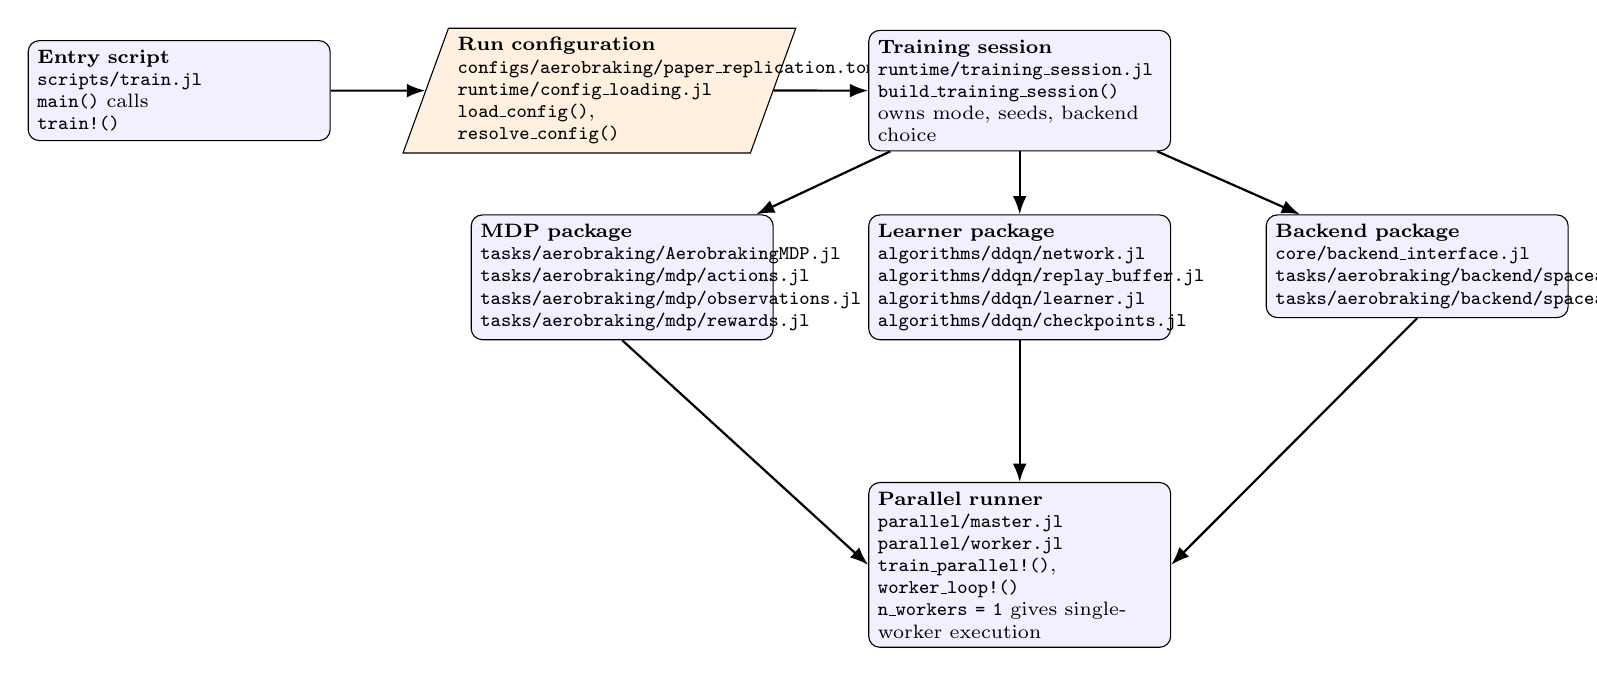
\begin{tikzpicture}[
    node distance=8mm and 12mm,
    >=Latex,
    font=\scriptsize,
    every node/.style={align=left},
    rl/.style={rectangle, draw, rounded corners, fill=blue!6, text width=36mm, minimum height=10mm},
    data/.style={trapezium, trapezium left angle=70, trapezium right angle=110, draw, fill=orange!12, text width=36mm, minimum height=10mm},
    line/.style={->, thick}
]
\node[rl] (script) {\textbf{Entry script}\\
    \texttt{scripts/train.jl}\\
    \texttt{main()} calls\\
    \texttt{train!()}};
\node[data, right=of script] (config) {\textbf{Run configuration}\\
    \texttt{configs/aerobraking/paper\_replication.toml}\\
    \texttt{runtime/config\_loading.jl}\\
    \texttt{load\_config()}, \texttt{resolve\_config()}};
\node[rl, right=of config] (session) {\textbf{Training session}\\
    \texttt{runtime/training\_session.jl}\\
    \texttt{build\_training\_session()}\\
    owns mode, seeds, backend choice};
\node[rl, below left=of session] (mdp) {\textbf{MDP package}\\
    \texttt{tasks/aerobraking/AerobrakingMDP.jl}\\
    \texttt{tasks/aerobraking/mdp/actions.jl}\\
    \texttt{tasks/aerobraking/mdp/observations.jl}\\
    \texttt{tasks/aerobraking/mdp/rewards.jl}};
\node[rl, below=of session] (learner) {\textbf{Learner package}\\
    \texttt{algorithms/ddqn/network.jl}\\
    \texttt{algorithms/ddqn/replay\_buffer.jl}\\
    \texttt{algorithms/ddqn/learner.jl}\\
    \texttt{algorithms/ddqn/checkpoints.jl}};
\node[rl, below right=of session] (backend) {\textbf{Backend package}\\
    \texttt{core/backend\_interface.jl}\\
    \texttt{tasks/aerobraking/backend/spaceagora\_backend.jl}\\
    \texttt{tasks/aerobraking/backend/spaceagora\_core\_adapter.jl}};
\node[rl, below=18mm of learner] (parallel) {\textbf{Parallel runner}\\
    \texttt{parallel/master.jl}\\
    \texttt{parallel/worker.jl}\\
    \texttt{train\_parallel!()}, \texttt{worker\_loop!()}\\
    \texttt{n\_workers = 1} gives single-worker execution};
\draw[line] (script) -- (config);
\draw[line] (config) -- (session);
\draw[line] (session) -- (mdp);
\draw[line] (session) -- (learner);
\draw[line] (session) -- (backend);
\draw[line] (mdp.south) -- (parallel.west);
\draw[line] (learner) -- (parallel);
\draw[line] (backend.south) -- (parallel.east);
\end{tikzpicture}%
}
\caption{Run setup. The \texttt{runtime/} files own config loading and session construction. The \texttt{parallel/} files own both single-worker and multi-worker execution through the same runner.}
\label{fig:spaceagora-rl-setup-flow}
\end{figure}

\subsection{Diagram 2: One Worker Decision Step}

\begin{figure}[h]
\centering
\resizebox{\textwidth}{!}{%
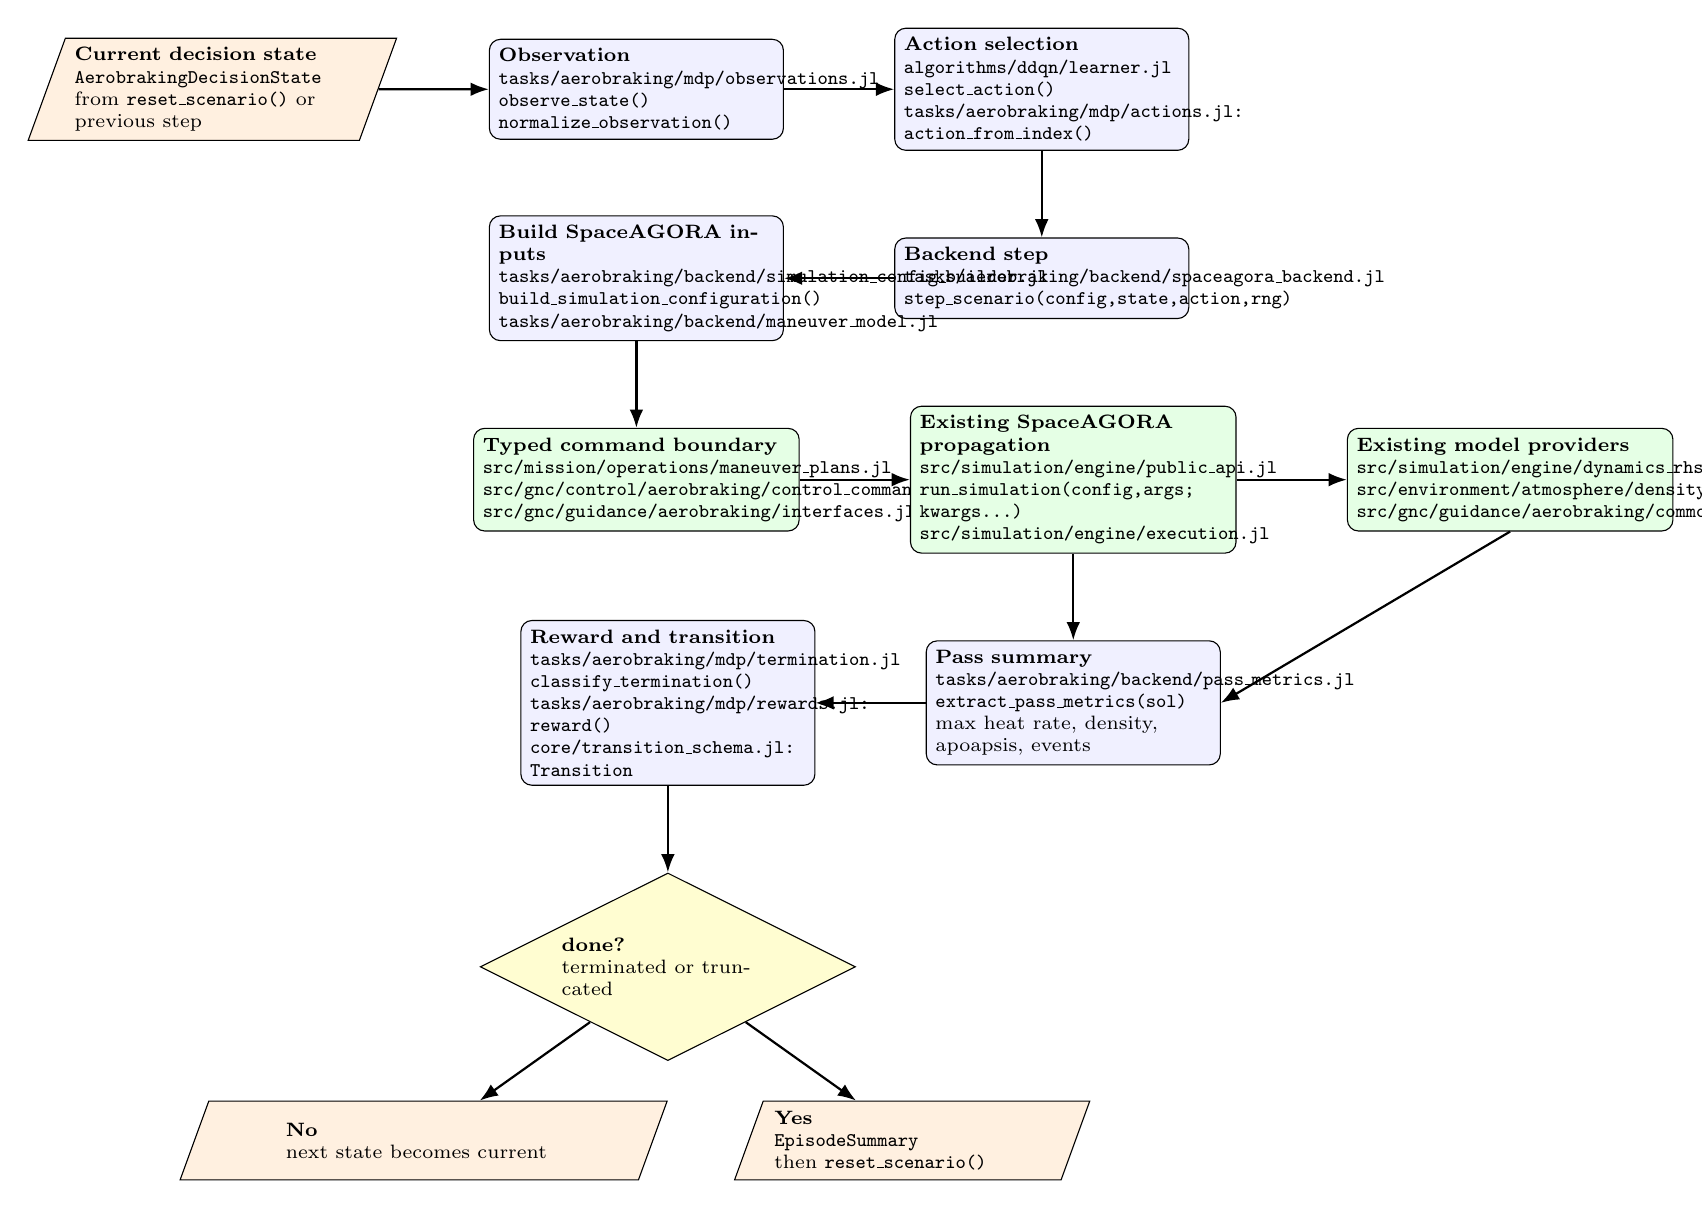
\begin{tikzpicture}[
    node distance=11mm and 14mm,
    >=Latex,
    font=\scriptsize,
    every node/.style={align=left},
    rl/.style={rectangle, draw, rounded corners, fill=blue!6, text width=35mm, minimum height=10mm},
    core/.style={rectangle, draw, rounded corners, fill=green!10, text width=39mm, minimum height=10mm},
    data/.style={trapezium, trapezium left angle=70, trapezium right angle=110, draw, fill=orange!12, text width=35mm, minimum height=10mm},
    decide/.style={diamond, draw, fill=yellow!18, aspect=2.0, text width=27mm, inner sep=1mm},
    line/.style={->, thick}
]
\node[data] (state) {\textbf{Current decision state}\\
    \texttt{AerobrakingDecisionState}\\
    from \texttt{reset\_scenario()} or previous step};
\node[rl, right=of state] (obs) {\textbf{Observation}\\
    \texttt{tasks/aerobraking/mdp/observations.jl}\\
    \texttt{observe\_state()}\\
    \texttt{normalize\_observation()}};
\node[rl, right=of obs] (action) {\textbf{Action selection}\\
    \texttt{algorithms/ddqn/learner.jl}\\
    \texttt{select\_action()}\\
    \texttt{tasks/aerobraking/mdp/actions.jl: action\_from\_index()}};
\node[rl, below=of action] (backendstep) {\textbf{Backend step}\\
    \texttt{tasks/aerobraking/backend/spaceagora\_backend.jl}\\
    \texttt{step\_scenario(config,state,action,rng)}};
\node[rl, left=of backendstep] (buildsim) {\textbf{Build SpaceAGORA inputs}\\
    \texttt{tasks/aerobraking/backend/simulation\_config\_builder.jl}\\
    \texttt{build\_simulation\_configuration()}\\
    \texttt{tasks/aerobraking/backend/maneuver\_model.jl}};
\node[core, below=of buildsim] (boundary) {\textbf{Typed command boundary}\\
    \texttt{src/mission/operations/maneuver\_plans.jl}\\
    \texttt{src/gnc/control/aerobraking/control\_commands.jl}\\
    \texttt{src/gnc/guidance/aerobraking/interfaces.jl}};
\node[core, right=of boundary] (runsim) {\textbf{Existing SpaceAGORA propagation}\\
    \texttt{src/simulation/engine/public\_api.jl}\\
    \texttt{run\_simulation(config,args; kwargs...)}\\
    \texttt{src/simulation/engine/execution.jl}};
\node[core, right=of runsim] (models) {\textbf{Existing model providers}\\
    \texttt{src/simulation/engine/dynamics\_rhs.jl}\\
    \texttt{src/environment/atmosphere/density\_models.jl}\\
    \texttt{src/gnc/guidance/aerobraking/common/heat\_rate\_models.jl}};
\node[rl, below=of runsim] (metrics) {\textbf{Pass summary}\\
    \texttt{tasks/aerobraking/backend/pass\_metrics.jl}\\
    \texttt{extract\_pass\_metrics(sol)}\\
    max heat rate, density, apoapsis, events};
\node[rl, left=of metrics] (transition) {\textbf{Reward and transition}\\
    \texttt{tasks/aerobraking/mdp/termination.jl}\\
    \texttt{classify\_termination()}\\
    \texttt{tasks/aerobraking/mdp/rewards.jl: reward()}\\
    \texttt{core/transition\_schema.jl: Transition}};
\node[decide, below=of transition] (done) {\textbf{done?}\\terminated or truncated};
\node[data, below left=of done] (continue) {\textbf{No}\\next state becomes current};
\node[data, below right=of done] (summary) {\textbf{Yes}\\
    \texttt{EpisodeSummary}\\
    then \texttt{reset\_scenario()}};
\draw[line] (state) -- (obs);
\draw[line] (obs) -- (action);
\draw[line] (action) -- (backendstep);
\draw[line] (backendstep) -- (buildsim);
\draw[line] (buildsim) -- (boundary);
\draw[line] (boundary) -- (runsim);
\draw[line] (runsim) -- (models);
\draw[line] (models.south) -- (metrics.east);
\draw[line] (runsim) -- (metrics);
\draw[line] (metrics) -- (transition);
\draw[line] (transition) -- (done);
\draw[line] (done) -- (continue);
\draw[line] (done) -- (summary);
\end{tikzpicture}%
}
\caption{One worker's environment step. The backend translates RL state/action into existing SpaceAGORA calls, then translates the resulting solution into pass metrics and MDP transition data. When \texttt{done} is false, the next state becomes the current state for the next decision. When \texttt{done} is true, the worker emits an episode summary and resets the scenario.}
\label{fig:spaceagora-rl-worker-step-flow}
\end{figure}

\subsection{Diagram 3: Master Learning and Artifacts}

\begin{figure}[htbp]
\centering
\resizebox{\textwidth}{!}{%
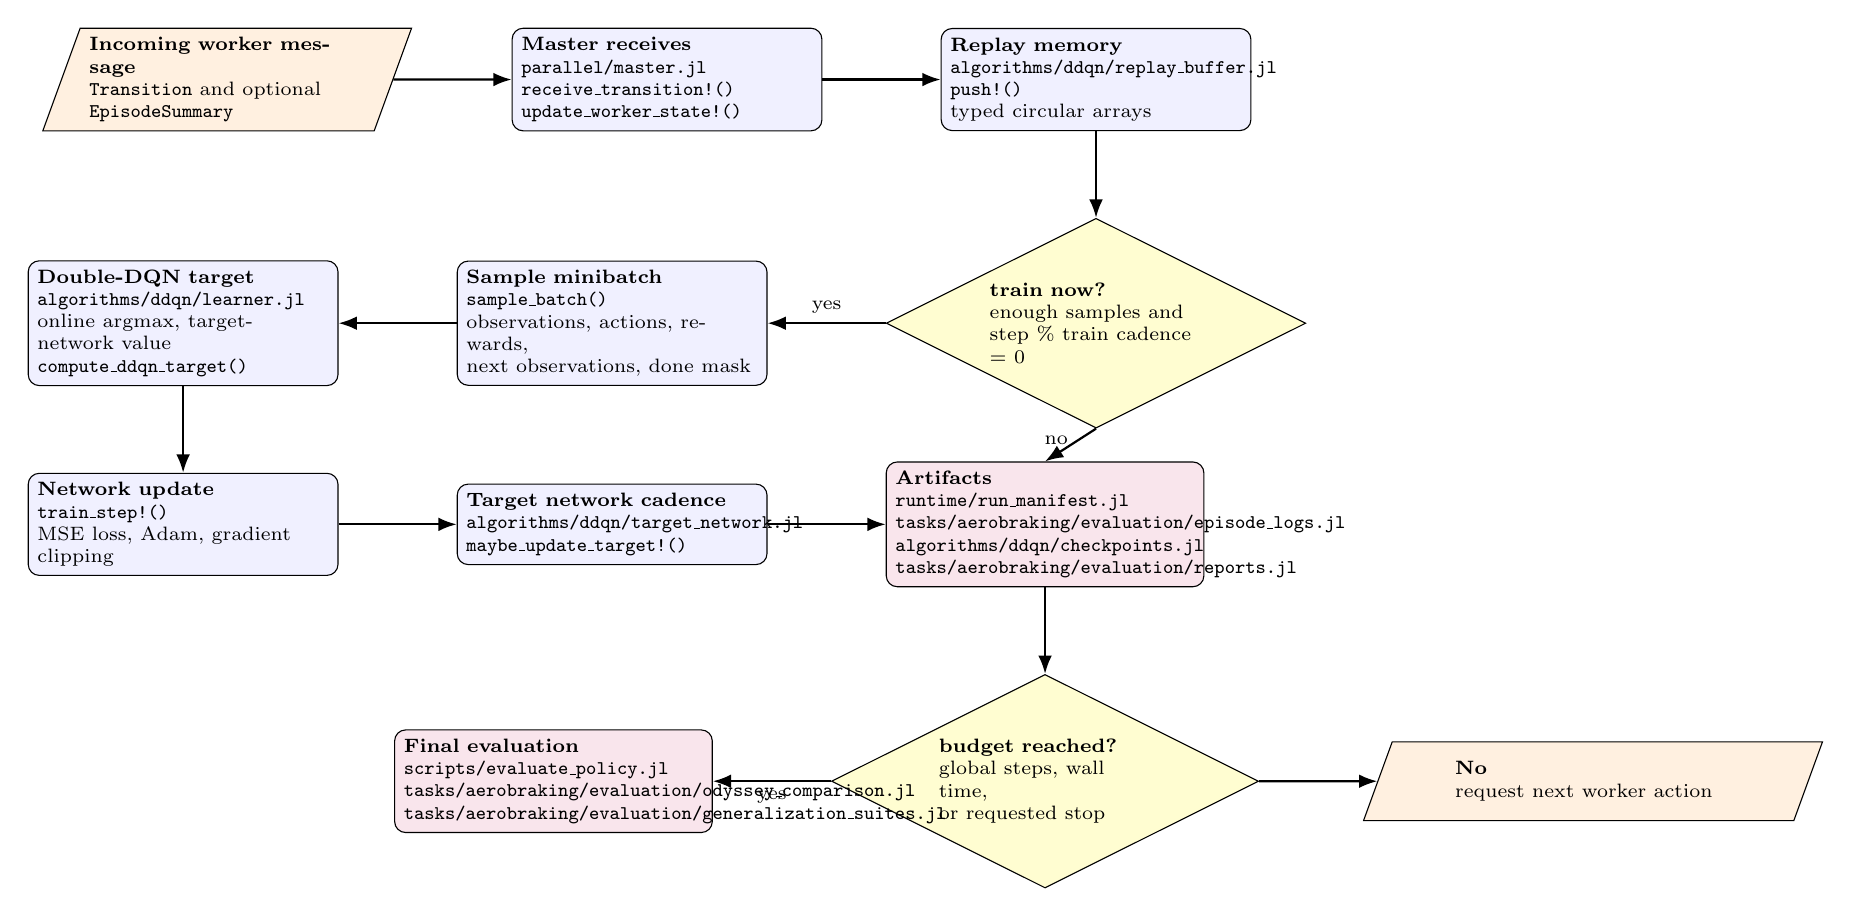
\begin{tikzpicture}[
    node distance=11mm and 15mm,
    >=Latex,
    font=\scriptsize,
    every node/.style={align=left},
    rl/.style={rectangle, draw, rounded corners, fill=blue!6, text width=37mm, minimum height=10mm},
    data/.style={trapezium, trapezium left angle=70, trapezium right angle=110, draw, fill=orange!12, text width=35mm, minimum height=10mm},
    artifact/.style={rectangle, draw, rounded corners, fill=purple!10, text width=38mm, minimum height=10mm},
    decide/.style={diamond, draw, fill=yellow!18, aspect=2.0, text width=27mm, inner sep=1mm},
    line/.style={->, thick}
]
\node[data] (incoming) {\textbf{Incoming worker message}\\
    \texttt{Transition} and optional\\
    \texttt{EpisodeSummary}};
\node[rl, right=of incoming] (receive) {\textbf{Master receives}\\
    \texttt{parallel/master.jl}\\
    \texttt{receive\_transition!()}\\
    \texttt{update\_worker\_state!()}};
\node[rl, right=of receive] (replay) {\textbf{Replay memory}\\
    \texttt{algorithms/ddqn/replay\_buffer.jl}\\
    \texttt{push!()}\\
    typed circular arrays};
\node[decide, below=of replay] (ready) {\textbf{train now?}\\
    enough samples and\\
    step \% train cadence = 0};
\node[rl, left=of ready] (batch) {\textbf{Sample minibatch}\\
    \texttt{sample\_batch()}\\
    observations, actions, rewards,\\
    next observations, done mask};
\node[rl, left=of batch] (target) {\textbf{Double-DQN target}\\
    \texttt{algorithms/ddqn/learner.jl}\\
    online argmax, target-network value\\
    \texttt{compute\_ddqn\_target()}};
\node[rl, below=of target] (update) {\textbf{Network update}\\
    \texttt{train\_step!()}\\
    MSE loss, Adam, gradient clipping};
\node[rl, right=of update] (targetnet) {\textbf{Target network cadence}\\
    \texttt{algorithms/ddqn/target\_network.jl}\\
    \texttt{maybe\_update\_target!()}};
\node[artifact, right=of targetnet] (artifacts) {\textbf{Artifacts}\\
    \texttt{runtime/run\_manifest.jl}\\
    \texttt{tasks/aerobraking/evaluation/episode\_logs.jl}\\
    \texttt{algorithms/ddqn/checkpoints.jl}\\
    \texttt{tasks/aerobraking/evaluation/reports.jl}};
\node[decide, below=of artifacts] (budget) {\textbf{budget reached?}\\global steps, wall time,\\or requested stop};
\node[artifact, left=of budget] (eval) {\textbf{Final evaluation}\\
    \texttt{scripts/evaluate\_policy.jl}\\
    \texttt{tasks/aerobraking/evaluation/odyssey\_comparison.jl}\\
    \texttt{tasks/aerobraking/evaluation/generalization\_suites.jl}};
\node[data, right=of budget] (continue_training) {\textbf{No}\\request next worker action};
\draw[line] (incoming) -- (receive);
\draw[line] (receive) -- (replay);
\draw[line] (replay) -- (ready);
\draw[line] (ready) -- node[above]{yes} (batch);
\draw[line] (batch) -- (target);
\draw[line] (target) -- (update);
\draw[line] (update) -- (targetnet);
\draw[line] (targetnet) -- (artifacts);
\draw[line] (ready.south) -- node[pos=0.35,left]{no} (artifacts.north);
\draw[line] (artifacts) -- (budget);
\draw[line] (budget) -- node[below]{yes} (eval);
\draw[line] (budget) -- (continue_training);
\end{tikzpicture}%
}
\caption{Master-side learning loop. Worker transitions enter replay; training and artifact writes are cadence-controlled so rollout, learning, checkpointing, and reporting remain separate concerns. The no-budget branch requests the next worker action and continues the same master loop.}
\label{fig:spaceagora-rl-master-learning-flow}
\end{figure}

\subsection{Run-Time Data Contract}

The flowchart preserves one data contract across execution:

\begin{enumerate}
\item \texttt{AerobrakingScenarioConfig} is built from \texttt{configs/aerobraking/paper\_replication.toml} and aerobraking backend scenario helpers.
\item \texttt{AerobrakingDecisionState} is the worker-owned state returned by \texttt{reset\_scenario} and updated by \texttt{step\_scenario}.
\item \texttt{AerobrakingAction} is created from the DDQN action index using \texttt{tasks/aerobraking/mdp/actions.jl}.
\item \texttt{AerobrakingStepResult} contains the next decision state, pass metrics, reward inputs, event flags, and termination/truncation flags.
\item \texttt{Transition} stores normalized observation, action index, reward, normalized next observation, terminal flags, and a compact info index.
\item \texttt{EpisodeSummary} stores pass count, mission duration, target error, thermal violation counts, total delta-V, maneuver count, heat-rate trace, action trace, and solver-failure flags.
\end{enumerate}



\section{Implementation Work Plan}

The implementation is completed as one integrated build of the SpaceAGORA RL system, based on this document, the reference code, and the Autonomous Decision-Making for Aerobraking via Parallel Randomized Deep Reinforcement Learning paper. The work items below are ordered by dependency, but they belong to the same implementation pass.

\subsection{Package and Runtime Setup}

\begin{itemize}
\item Create \texttt{SpaceAGORA\_RL.jl/Project.toml} and \texttt{SpaceAGORA\_RL.jl/src/SpaceAGORA\_RL.jl}.
\item Add \texttt{core/mdp\_interface.jl}, \texttt{core/backend\_interface.jl}, \texttt{core/policy\_interface.jl}, and \texttt{core/transition\_schema.jl} for task-independent interfaces and data contracts.
\item Add \texttt{runtime/config\_loading.jl} for TOML parsing and resolved configuration construction.
\item Add \texttt{runtime/training\_session.jl} for seed ownership, run-mode selection, backend construction, and learner construction.
\item Add \texttt{runtime/run\_manifest.jl} for recording package versions, git commits, manifests, solver settings, reward settings, normalization settings, and random seeds.
\item Keep generated training products under \texttt{outputs/}; commit only \texttt{outputs/.gitkeep}.
\end{itemize}

\subsection{Aerobraking Task MDP and Configuration}

\begin{itemize}
\item Implement \texttt{tasks/aerobraking/AerobrakingMDP.jl} as the aerobraking task module that wires the task-specific MDP, backend, baselines, and evaluation files into the generic interfaces.
\item Implement \texttt{tasks/aerobraking/mdp/actions.jl} with the 13 paper actions, action-index mapping, and sign convention.
\item Implement \texttt{tasks/aerobraking/mdp/observations.jl} with the raw paper observation, normalized observation vector, schema metadata, and checkpoint metadata.
\item Implement \texttt{tasks/aerobraking/mdp/normalization.jl} with the normalization bounds from the reference code.
\item Implement \texttt{tasks/aerobraking/mdp/rewards.jl} with the paper reward profile and TOML-backed reward parameters.
\item Implement \texttt{tasks/aerobraking/mdp/termination.jl} with target, undershoot, impact, out-of-passage, and thermal violation classification.
\item Implement \texttt{tasks/aerobraking/mdp/randomization.jl} with initial-condition and environment randomization parameters used by the backend.
\item Include Main, Walkout, Endgame, and Campaign scenario constants in the resolved configuration.
\item Store aerobraking run configurations under \texttt{configs/aerobraking/}.
\end{itemize}

\subsection{Aerobraking SpaceAGORA Backend}

\begin{itemize}
\item Use \texttt{core/backend\_interface.jl} for the generic backend contract.
\item Implement aerobraking backend types, including \texttt{AerobrakingScenarioConfig}, \texttt{AerobrakingDecisionState}, \texttt{AerobrakingAction}, \texttt{AerobrakingPassMetrics}, and \texttt{AerobrakingStepResult}, under \texttt{tasks/aerobraking/backend/}.
\item Implement \texttt{tasks/aerobraking/backend/spaceagora\_backend.jl} as the backend facade exposing \texttt{reset\_scenario(config, rng)} and \texttt{step\_scenario(config, state, action, rng)}.
\item Implement \texttt{tasks/aerobraking/backend/simulation\_config\_builder.jl} to translate an RL scenario state and action into the typed SpaceAGORA simulation configuration used by \texttt{run\_simulation}.
\item Implement \texttt{tasks/aerobraking/backend/spaceagora\_core\_adapter.jl} for calls into existing SpaceAGORA APIs, including \texttt{src/simulation/engine/public\_api.jl} and \texttt{src/simulation/engine/execution.jl}.
\item Implement \texttt{tasks/aerobraking/backend/maneuver\_model.jl} to convert the discrete RL delta-V action into the typed maneuver or command representation used at the SpaceAGORA boundary.
\item Implement \texttt{tasks/aerobraking/backend/pass\_metrics.jl} to extract apoapsis radius, periapsis altitude, orbital angles, drag-passage duration, date/season feature, maximum density, maximum heat rate, event flags, solver status, maneuver count, and total delta-V from the SpaceAGORA result.
\item Keep optional paper heat-rate parity code isolated in \texttt{tasks/aerobraking/backend/paper\_heat\_rate\_metrics.jl} if the study requires a paper-mode evaluator distinct from SpaceAGORA native heat-rate metrics.
\end{itemize}

\subsection{DDQN Learner}

\begin{itemize}
\item Implement \texttt{algorithms/ddqn/network.jl} as a Flux Q-network with paper-mode input dimension 9, two 1024-unit hidden layers, ReLU activations, and 13 action outputs.
\item Implement \texttt{algorithms/ddqn/replay\_buffer.jl} as a typed circular replay buffer using contiguous arrays.
\item Implement \texttt{algorithms/ddqn/epsilon\_schedule.jl} with the configured exploration schedule.
\item Implement \texttt{algorithms/ddqn/learner.jl} with action selection, transition ingestion, Double-DQN target calculation, MSE loss, Adam updates, gradient clipping, and training cadence control.
\item Implement \texttt{algorithms/ddqn/target\_network.jl} with configured target-network update cadence.
\item Implement \texttt{algorithms/ddqn/checkpoints.jl} with checkpoint save/load for model weights, optimizer state, action table, normalization schema, reward configuration, run manifest, and global step.
\end{itemize}

\subsection{Parallel Runner}

\begin{itemize}
\item Use \texttt{core/transition\_schema.jl} for \texttt{Transition} and \texttt{EpisodeSummary}.
\item Implement \texttt{parallel/master.jl} with \texttt{train\_parallel!()}, transition receipt, replay insertion, learner updates, checkpoint cadence, metrics updates, and worker action dispatch.
\item Implement \texttt{parallel/worker.jl} with \texttt{worker\_loop!()}, worker-local backend state, worker-local RNG, scenario reset, decision-step execution, and episode-summary emission.
\item Implement \texttt{parallel/distributed\_backend.jl} with Julia \texttt{Distributed} process setup. The same runner is used for single-worker execution by setting \texttt{n\_workers = 1}.
\item Keep the transition schema identical for \texttt{n\_workers = 1} and \texttt{n\_workers > 1}.
\end{itemize}

\subsection{Baselines, Evaluation, and Reports}

\begin{itemize}
\item Implement \texttt{tasks/aerobraking/baselines/no\_maneuver.jl}, \texttt{tasks/aerobraking/baselines/random\_policy.jl}, \texttt{tasks/aerobraking/baselines/fixed\_corridor.jl}, and \texttt{tasks/aerobraking/baselines/aads\_heuristic.jl} against the same SpaceAGORA backend contract.
\item Implement \texttt{tasks/aerobraking/evaluation/metrics.jl} for success rate, final target error, thermal violation counts, total delta-V, maneuver count, pass count, mission duration, peak heat rate, minimum periapsis, and solver-failure counts.
\item Implement \texttt{tasks/aerobraking/evaluation/episode\_logs.jl} for structured episode records.
\item Implement \texttt{tasks/aerobraking/evaluation/odyssey\_comparison.jl}, \texttt{tasks/aerobraking/evaluation/generalization\_suites.jl}, and \texttt{tasks/aerobraking/evaluation/reports.jl} for replication and generalization reporting.
\item Implement \texttt{scripts/train.jl}, \texttt{scripts/evaluate\_policy.jl}, \texttt{scripts/run\_baselines.jl}, and \texttt{scripts/run\_generalization\_suite.jl} using the same config resolver and backend contract.
\end{itemize}


\subsection{Examples}

\begin{itemize}
\item Implement \texttt{examples/aerobraking/example\_SpaceAGORA\_RL\_MarsOdyssey.jl} to run the main aerobraking example.
\item Keep \texttt{examples/future\_tasks/README.md} as the placeholder for adding non-aerobraking examples under sibling example namespaces.
\end{itemize}


\subsection{Acceptance Criteria}

\begin{itemize}
\item \texttt{julia --project=SpaceAGORA\_RL.jl -e 'using SpaceAGORA\_RL'} loads the package.
\item The resolved paper-replication configuration contains the action table, normalization map, reward profile, backend settings, worker settings, randomization settings, and report settings.
\item A fixed seed with \texttt{n\_workers = 1} produces reproducible pass summaries and transition logs through the SpaceAGORA backend.
\item A fixed seed with \texttt{n\_workers > 1} records worker seeds, transition counts, episode summaries, and run manifest entries.
\item DDQN target calculation, replay-buffer wraparound, action mapping, normalization, reward, and termination tests pass.
\item Checkpoints round-trip model weights, optimizer state, action table, normalization schema, reward configuration, and run manifest.
\item Baseline and learned-policy evaluations emit the same metric schema.
\item Generated artifacts are written under \texttt{outputs/} and are excluded from source control except for placeholders.
\end{itemize}

\section{Test Coverage}

\begin{enumerate}
\item \texttt{action\_table\_is\_ordered\_and\_signed}
\begin{itemize}
\item Confirms 13 actions.
\item Confirms Python index 6 maps to Julia index 7 zero action.
\item Confirms negative action lowers periapsis convention.

\end{itemize}
\item \texttt{paper\_observation\_normalization\_matches\_reference}
\begin{itemize}
\item Uses representative raw observation values.
\item Checks normalized vector order:
drag time, apoapsis radius, periapsis altitude, omega, RAAN, inclination, date, density, heat rate.

\end{itemize}
\item \texttt{thermal\_violation\_classes\_are\_exclusive}
\begin{itemize}
\item Low, nominal, high, soft, medium, hard.

\end{itemize}
\item \texttt{reward\_matches\_reference\_cases}
\begin{itemize}
\item In-corridor running reward.
\item Low heat-rate penalty while far from target.
\item 0.30 to 0.45 W/cm\textasciicircum{}2 penalty.
\item Greater than 0.45 W/cm\textasciicircum{}2 penalty.
\item Success terminal reward.
\item Target undershoot penalty.

\end{itemize}
\item \texttt{replay\_buffer\_wraparound}
\begin{itemize}
\item Push more than capacity.
\item Sample minibatch.
\item Confirm no shape instability.

\end{itemize}
\item \texttt{ddqn\_target\_uses\_online\_argmax\_and\_target\_value}
\begin{itemize}
\item Hand-set Q values and target Q values.
\item Confirm Double-DQN target.

\end{itemize}
\item \texttt{spaceagora\_backend\_rollout\_is\_seed\_reproducible}
\begin{itemize}
\item Same seed, same config, same action trace, same SpaceAGORA pass metrics.


\end{itemize}
\end{enumerate}
\section{Concrete Files to Create or Update}

\paragraph{Create.}

\begin{itemize}
\item \texttt{SpaceAGORA\_RL.jl/Project.toml}
\item \texttt{SpaceAGORA\_RL.jl/src/SpaceAGORA\_RL.jl}
\item \texttt{SpaceAGORA\_RL.jl/src/core/mdp\_interface.jl}
\item \texttt{SpaceAGORA\_RL.jl/src/core/backend\_interface.jl}
\item \texttt{SpaceAGORA\_RL.jl/src/core/policy\_interface.jl}
\item \texttt{SpaceAGORA\_RL.jl/src/core/transition\_schema.jl}
\item \texttt{SpaceAGORA\_RL.jl/src/runtime/config\_loading.jl}
\item \texttt{SpaceAGORA\_RL.jl/src/runtime/run\_manifest.jl}
\item \texttt{SpaceAGORA\_RL.jl/src/runtime/training\_session.jl}
\item \texttt{SpaceAGORA\_RL.jl/src/algorithms/ddqn/replay\_buffer.jl}
\item \texttt{SpaceAGORA\_RL.jl/src/algorithms/ddqn/network.jl}
\item \texttt{SpaceAGORA\_RL.jl/src/algorithms/ddqn/epsilon\_schedule.jl}
\item \texttt{SpaceAGORA\_RL.jl/src/algorithms/ddqn/learner.jl}
\item \texttt{SpaceAGORA\_RL.jl/src/algorithms/ddqn/target\_network.jl}
\item \texttt{SpaceAGORA\_RL.jl/src/algorithms/ddqn/checkpoints.jl}
\item \texttt{SpaceAGORA\_RL.jl/src/parallel/rollout\_protocol.jl}
\item \texttt{SpaceAGORA\_RL.jl/src/parallel/master.jl}
\item \texttt{SpaceAGORA\_RL.jl/src/parallel/worker.jl}
\item \texttt{SpaceAGORA\_RL.jl/src/parallel/distributed\_backend.jl}
\item \texttt{SpaceAGORA\_RL.jl/src/tasks/aerobraking/AerobrakingMDP.jl}
\item \texttt{SpaceAGORA\_RL.jl/src/tasks/aerobraking/mdp/actions.jl}
\item \texttt{SpaceAGORA\_RL.jl/src/tasks/aerobraking/mdp/observations.jl}
\item \texttt{SpaceAGORA\_RL.jl/src/tasks/aerobraking/mdp/normalization.jl}
\item \texttt{SpaceAGORA\_RL.jl/src/tasks/aerobraking/mdp/rewards.jl}
\item \texttt{SpaceAGORA\_RL.jl/src/tasks/aerobraking/mdp/termination.jl}
\item \texttt{SpaceAGORA\_RL.jl/src/tasks/aerobraking/mdp/randomization.jl}
\item \texttt{SpaceAGORA\_RL.jl/src/tasks/aerobraking/backend/spaceagora\_backend.jl}
\item \texttt{SpaceAGORA\_RL.jl/src/tasks/aerobraking/backend/simulation\_config\_builder.jl}
\item \texttt{SpaceAGORA\_RL.jl/src/tasks/aerobraking/backend/spaceagora\_core\_adapter.jl}
\item \texttt{SpaceAGORA\_RL.jl/src/tasks/aerobraking/backend/maneuver\_model.jl}
\item \texttt{SpaceAGORA\_RL.jl/src/tasks/aerobraking/backend/pass\_metrics.jl}
\item \texttt{SpaceAGORA\_RL.jl/src/tasks/aerobraking/baselines/aads\_heuristic.jl}
\item \texttt{SpaceAGORA\_RL.jl/src/tasks/aerobraking/evaluation/metrics.jl}
\item \texttt{SpaceAGORA\_RL.jl/configs/aerobraking/paper\_replication.toml}
\item \texttt{SpaceAGORA\_RL.jl/tests/runtests.jl}
\end{itemize}

\paragraph{SpaceAGORA core updates.}

\begin{itemize}
\item \texttt{src/mission/operations/aerobraking\_policy/selector\_stub.jl}
\begin{itemize}
\item Keep current throwing stub for unimplemented policy.
\item Later add a concrete adapter only after the policy artifact and typed input/output are known.

\end{itemize}
\item \texttt{src/gnc/control/aerobraking/control\_commands.jl}
\begin{itemize}
\item Use existing typed command boundary.
\item Add fields only if the generalized mode requires a periapsis/corridor target that is not representable.
\end{itemize}
\end{itemize}

\paragraph{Unchanged SpaceAGORA areas.}

\begin{itemize}
\item Existing guidance solvers.
\item Existing control/tracking internals.
\item Simulation engine hot paths.
\item GRAM/SPICE global-state handling.
\end{itemize}



\section{Implementation Scope Summary}

The implementation consists of a Julia-native \texttt{SpaceAGORA\_RL.jl} package with:

\begin{itemize}
\item reusable core interfaces for MDPs, backend adapters, policies, and transitions;
\item paper-faithful aerobraking MDP definitions for actions, observations, normalization, reward, and termination;
\item an aerobraking SpaceAGORA backend facade for reset and decision-step execution;
\item reusable DDQN learner, replay buffer, target-network update, epsilon schedule, and checkpoints;
\item one parallel runner that supports \texttt{n\_workers = 1} and \texttt{n\_workers > 1};
\item aerobraking baseline policies and evaluation/reporting tools;
\item task-namespaced configuration modes for paper replication and SpaceAGORA-native/MPC generalization.
\end{itemize}

The SpaceAGORA core remains responsible for simulation, dynamics, atmosphere, heat-rate calculation, guidance/control boundaries, and solver execution. The RL package calls SpaceAGORA through task-specific backend facades and records the resulting metrics, transitions, checkpoints, and reports. Future non-aerobraking examples are added as sibling task namespaces under \texttt{tasks/}, \texttt{configs/}, \texttt{tests/tasks/}, and \texttt{examples/}.

\end{document}
